\documentclass[12pt, a4paper, twoside, titlepage]{article}
\usepackage[brazilian]{babel}
\usepackage[utf8]{inputenc}
\usepackage[T1]{fontenc}
\usepackage{import}
\usepackage[pdftex]{graphicx}
\usepackage{fancyhdr}
\usepackage{listings}
\usepackage{color}

\definecolor{dkgreen}{rgb}{0,0.6,0}
\definecolor{gray}{rgb}{0.5,0.5,0.5}
\definecolor{mauve}{rgb}{0.58,0,0.82}

\lstset{frame=tb,
  language=Python,
  aboveskip=3mm,
  belowskip=3mm,
  showstringspaces=false,
  columns=flexible,
  basicstyle={\small\ttfamily},
  numbers=none,
  numberstyle=\tiny\color{gray},
  keywordstyle=\color{blue},
  commentstyle=\color{dkgreen},
  stringstyle=\color{mauve},
  breaklines=true,
  breakatwhitespace=true,
  tabsize=3
}


%%% Custom headers/footers (fancyhdr package)
\pagestyle{fancyplain}
\fancyhead{}											% No page header
\fancyfoot[L]{}											% Empty
\fancyfoot[C]{}											% Empty
\fancyfoot[R]{\thepage}									% Pagenumbering
\renewcommand{\headrulewidth}{0pt}			% Remove header underlines
\renewcommand{\footrulewidth}{0pt}				% Remove footer underlines
\setlength{\headheight}{13.6pt}

%%% Maketitle metadata
\newcommand{\horrule}[1]{\rule{\linewidth}{#1}} 	% Horizontal rule

\title{
		\normalfont \normalsize \textsc{Universidade Estadual de Santa Cruz} \\ [25pt]
		\horrule{0.5pt} \\[0.4cm]
		\huge Relação entre o número de Clientes e Transações por cliente\\
		\horrule{2pt} \\[0.5cm]
}

\author{
	\normalfont 								\normalsize
	Eduardo Reis Nobre\\[-3pt]		\normalsize
}

\begin{document}

\maketitle


% \begin{abstract}
% \end{abstract}

\tableofcontents % create a table of contens
\clearpage

\section{Introdução}
Durante a implementação de um banco de dados, devemos considerar que tipo de aplicação teremos e se a máquina escolhida para o serviço é capaz de atender a aplicação. A capacidade de simular cenários e ver como sua máquina reagirá a tais cenários pode ser obtida de duas formas: através de uso real, onde se utilizará uma configuração média sendo armazenado as informações relevantes ou através de uma ferramenta de benchmark que é capaz de realizar diversos testes em diversos cenários sem a necessidade da interação com usuário lhe dando o controle sobre diversos aspectos da simulação. Esse relatório fala do uso do pgbench para a o teste de performance do banco de dados postgres.
\section{Ambiente}
Os testes foram realizados utilizando um computador com a seguinte configuração:\\\\
\textbf{\textbf{}Processador:} Intel Core i7 3770 @ 3.40GHz x 4\\
\textbf{\textbf{}Memória Ram:} 8Gb @ 1600MHz\\
\textbf{HD:} Western Digital 500gb, Leitura 176 MB/s, Escrita 167MB/s\\
\textbf{SO:} Linux Mint 18.2 Cinnamon 64 bits.

Os testes foram realizados utilizando-se o sgbd postgres versão 9.5.

\section{Metodologia} \label{documentclasses}
Todos os cenários foram testados 10 vezes, sendo obtidas então as médias de Latência e quantidade de transações por segundo. As chamadas foram realizadas para um banco com um fator de escala de 10 utilizando um script em python3 para a realização das chamadas, cálculo e armazenamento dos resultados para posterior análise.
\\O script realiza um teste cruzado dentro de um vetor de quantidades tanto para clientes quanto para transações por clientes. Ambos vetores possuem a seguinte estrutura [1, 15, 30, 45, 60, 75, 90, 100]. Dois loops se encarregam de testar todas as combinações de clientes e transações possíveis, combinando então, 1 cliente com 1 transação, 1 cliente com 15 transações e assim por diante, sendo que para cada combinação, também chamada de cenário, 10 testes são realizados para evitar valores que não representem a realidade.
\\
\begin{lstlisting}
BATCH_SIZE = 10
CLIENTS = [5, 15, 30, 45, 60, 75, 90, 100]
TRANSACTIONS = [1, 15, 30, 45, 60, 75, 90, 100]

def make_csv_batch(client=10, transaction=10):
    body = ''
    lines = ''
    for index in range(1, BATCH_SIZE+1):
        process = subprocess.Popen('pgbench -d -C -c {} -t {} benchmark'.format(client, transaction).split(), stdout=subprocess.PIPE)
        output, error = process.communicate()
        line = output.decode().split('\n')[8:12]
        lines = lines + make_csv_line(line)
    
    body = body + make_mean(lines) 
    with open(OUT_PATH + 'out_t5_{}x{}.csv'.format(client, transaction), 'w') as outfile:
        outfile.write(body)

def make():
    for client in CLIENTS:
        for transaction in TRANSACTIONS:
            make_csv_batch(client, transaction)

\end{lstlisting}
\\Os resultados são tratados por uma função e convertidos em uma um vetor de valores e então armazenados em um vetor acumulador. Ao fim dos 10 testes, é realizada uma média dos valores acumulados, sendos escritos em formato csv em uma pasta de saídas, dando seguimento então para o próximo cenário.
\\Após o processo de coleta de dados, é executado um outro script sendo passado na chamadas do script uma lista de arquivos a serem analisados.\\
\\O próximo teste foi realizado utilizando o modificador -j que realiza a transações utilizando-se threads utilizado alterando-se a flag -f. Os testes foram realizados utilizando 5 threads. O vetor de valores de clientes teve de ser alterado pois todos os valores do cenário devem ser múltiplos do número de threads.
\begin{lstlisting}
CLIENTS = [5, 15, 30, 45, 60, 75, 90, 100]

def make_csv_batch(client=10, transaction=10):
	# stuff above
    process = subprocess.Popen('pgbench -d -C -c {} -t {} -j 5 benchmark'.format(client, transaction).split(), stdout=subprocess.PIPE)
	# stuff below
\end{lstlisting}

% \begin{itemize}
% \item article
% \item book
% \item report
% \item letter
% \end{itemize}
%
%
% \begin{enumerate}
% \item article
% \item book
% \item report
% \item letter
% \end{enumerate}

% \begin{description}
% \item[article\label{article}]{Article is \ldots}
% \item[book\label{book}]{The book class \ldots}
% \item[report\label{report}]{Report gives you \ldots}
% \item[letter\label{letter}]{If you want to write a letter.}
% \end{description}

\section{Resultados}
Na média de testes para 1 cliente, tem um resultado que difere dos outros cenários, onde ocorrem mais clientes são simulados, os tempos são relativamente baixos, já que apenas 1 cliente está realizando operações no sistemas. Os tempos variam de forma não linear com um desvio padrão de 0.0435. É possível se observar pouca ou nenhuma relação entre os tempos a quantidade transações de -0.26.
\begin{figure}[!htb]
	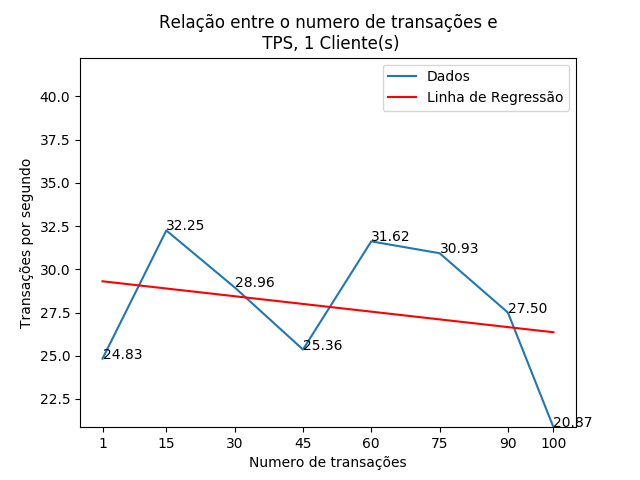
\includegraphics[width=\textwidth]{imgs/1_client.png}
	\caption{Relação entre o número de transções por clientes e a quantidade de transações por segundo}
\end{figure}

\\Ao aumentarmos a quantidade de clientes realizando as conexões podemos notar um aumento no número de transações por segundo, isso já era esperado já que tempos um número maior de transações realizadas, porém algo inesperado foi que a correlação entre as variáveis observadas não se tornou mais forte. Isso pode ter sido causado por conta do sistema não ter sido submetido a um cenário que chegasse próximo ao seu limite, fazendo com que ele operasse constantemente abaixo da sua capacidade, não mostrando assim nenhum resultado relevante.
\\Graficamente, fora os casos onde são testados 30 clientes e 75 clientes, os gráficos tem o mesmo comportamento geral, onde inicialmente ele apresenta um comportamento decrescente, caindo rapidamente e se estabilizando, porém a correlação entre variáveis se mantém baixa.
\\\\Assim como nos testes realizados utilizando apenas uma thread, os coeficientes de correlação se mantiveram baixos, apesar do número de transações por segundo ter aumentado em basicamente todos os cenários.
\\\\O código utilizado, assim como os detalhes para cada um dos cenários se encontra no repostiório a seguir: \href{https://github.com/reisnobre/db_2_benchmark}{Github} 
\end{document}
